% !TeX program = lualatex
% !TeX encoding = UTF-8
\documentclass[10pt]{article}
\usepackage[landscape,a4paper]{geometry}
\usepackage{tikz}
\usepackage{xcolor}
\usepackage{parskip}
\usepackage{multicol}
\usepackage{amsmath}
\usepackage{pgfplots}
\pgfplotsset{compat=1.18}

% Use standard fonts to avoid Arial issues
\usepackage[T1]{fontenc}
\usepackage[default]{sourcesanspro}
\usepackage{helvet}

% Dark theme colors inspired by formulasheet
\definecolor{darkbg}{HTML}{222222}
\definecolor{lighttext}{HTML}{eeeeee}

% Month-specific colors
\definecolor{coljan}{HTML}{FFBFFF}
\definecolor{colfeb}{HTML}{BFFFFF}
\definecolor{colmar}{HTML}{BFFFBF}
\definecolor{colapr}{HTML}{FFFFBF}
\definecolor{colmay}{HTML}{FFDFBF}
\definecolor{coljun}{HTML}{DFBFFF}
\definecolor{coljul}{HTML}{BFFFDF}
\definecolor{colaug}{HTML}{FFBFDF}
\definecolor{colsep}{HTML}{DFFFBF}
\definecolor{coloct}{HTML}{BFDFFF}
\definecolor{colnov}{HTML}{FFDFFF}
\definecolor{coldec}{HTML}{DFDFFF}

\geometry{
    top=0.5in,
    bottom=0.5in,
    left=0.25in,
    right=0.25in
}

\pagestyle{empty}
\pagecolor{darkbg}
\color{lighttext}

\newcommand{\monthname}[1]{%
    \ifcase#1\relax\or January\or February\or March\or April\or May\or June\or
    July\or August\or September\or October\or November\or December\fi
}

% Function to get month color
\newcommand{\monthcolor}[1]{%
    \ifcase#1\relax%
    \or coljan\or colfeb\or colmar\or colapr\or colmay\or coljun%
    \or coljul\or colaug\or colsep\or coloct\or colnov\or coldec%
    \fi%
}

\newcommand{\daysofmonth}[2]{%
    \ifcase#2\relax\or
        31\or
        \ifnum#1=2000 29\else\ifnum\numexpr#1/4*4=#1 29\else 28\fi\fi\or
        31\or 30\or 31\or 30\or 31\or 31\or 30\or 31\or 30\or 31
    \fi
}

% Calculate day of week for first day of month (0=Sun, 1=Mon, etc.)
% Using Zeller's Congruence for 2026
\newcommand{\firstdayofmonth}[1]{%
    \ifcase#1\relax\or
        4\or  % Jan 1, 2026 = Thursday (4)
        0\or  % Feb 1, 2026 = Sunday (0)
        0\or  % Mar 1, 2026 = Sunday (0)
        3\or  % Apr 1, 2026 = Wednesday (3)
        5\or  % May 1, 2026 = Friday (5)
        1\or  % Jun 1, 2026 = Monday (1)
        3\or  % Jul 1, 2026 = Wednesday (3)
        6\or  % Aug 1, 2026 = Saturday (6)
        2\or  % Sep 1, 2026 = Tuesday (2)
        4\or  % Oct 1, 2026 = Thursday (4)
        0\or  % Nov 1, 2026 = Sunday (0)
        2     % Dec 1, 2026 = Tuesday (2)
    \fi%
}

\newcommand{\calendarheader}[1]{%
    \begin{tikzpicture}[remember picture, overlay]
        \node[anchor=north west, inner sep=0pt, outer sep=0pt] 
            at (current page.north west)
            {\begin{tikzpicture}
                \fill[\monthcolor{#1}] (0,0) rectangle (\paperwidth, 0.5cm);
                \node[anchor=west, text=darkbg, font=\bfseries\Large, xshift=1.25cm] 
                    at (0,0.25) {Year 2026};
                \node[anchor=east, text=darkbg, font=\bfseries\Large, xshift=-1.25cm] 
                    at (\paperwidth,0.25) {Calendar};
            \end{tikzpicture}};
    \end{tikzpicture}
}

\newcommand{\monthcalendar}[1]{%
    \begin{tikzpicture}
        % Month header
        \fill[\monthcolor{#1}] (0,0) rectangle (7.7, 0.9);
        \node[anchor=west, font=\bfseries\huge, text=darkbg]
            at (0,0.3) {\monthname{#1}};

        % Day headers
        \foreach \day[count=\i] in {Sun, Mon, Tue, Wed, Thu, Fri, Sat} {
            \node[anchor=center, font=\bfseries\large, text=lighttext]
                at ({(\i-0.6)*1.1}, -1) {\day};
        }

        % Days grid
        \pgfmathsetmacro{\totaldays}{\daysofmonth{2026}{#1}}
        \pgfmathsetmacro{\startday}{\firstdayofmonth{#1}}
        \foreach \row in {0,...,5} {
            \foreach \col in {0,...,6} {
                \pgfmathsetmacro{\daynum}{int(\row*7 + \col - \startday + 1)}
                \ifnum\daynum>0
                    \ifnum\daynum<\totaldays
                        \node[draw=\monthcolor{#1}!50, thick, fill=darkbg!80,
                              minimum width=0.95cm, minimum height=0.95cm,
                              text=lighttext, font=\bfseries\normalsize]
                            at ({\col*1.1 + 0.5}, {-\row*1.1 - 1.8})
                            {\daynum};
                    \else
                        \ifnum\daynum=\totaldays
                            \node[draw=\monthcolor{#1}, thick, fill=\monthcolor{#1}!20,
                                  minimum width=0.95cm, minimum height=0.95cm,
                                  text=lighttext, font=\bfseries\small]
                                at ({\col*1.1 + 0.5}, {-\row*1.1 - 1.8})
                                {\daynum};
                        \fi
                    \fi
                \fi
            }
        }
    \end{tikzpicture}
    \vspace{0.3cm}
}

\begin{document}

% Title Page
\begin{center}
	\vspace*{2cm}
	
\begin{tikzpicture}
		\fill[coljan] (0,0) rectangle (0.8\paperwidth, 1.5cm);
		\node[anchor=center, font=\bfseries\Huge, text=darkbg]
		at (0.4\paperwidth, 0.75cm) {2026 CALENDAR};
	\end{tikzpicture}

	\vspace{1.5cm}

	% Simple month blocks
	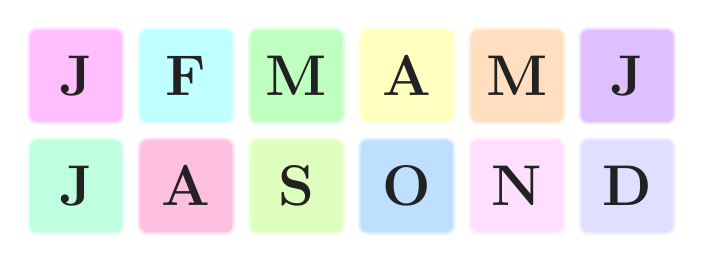
\begin{tikzpicture}
		\foreach \m[count=\i] in {J,F,M,A,M,J,J,A,S,O,N,D} {
				\pgfmathsetmacro{\xpos}{mod(\i-1,6)*1.4}
				\pgfmathsetmacro{\ypos}{-int((\i-1)/6)*1.4}
				\node[anchor=center, fill=\monthcolor{\i},
					draw=\monthcolor{\i}!50, thick,
					minimum width=1.2cm, minimum height=1.2cm,
					text=darkbg, font=\bfseries\huge,
					rounded corners=3pt
				]
				at (\xpos, \ypos) {\m};
			}
	\end{tikzpicture}

	\vfill

	\textcolor{lighttext}{\Large Made by Harshit Dhanwalkar}

	\vspace{1.5cm}

	
\begin{tikzpicture}
		\draw[colmar, very thick] (0,0) -- (0.5\paperwidth,0);
	\end{tikzpicture}

	\vspace{1cm}
\end{center}

\pagebreak

% January-February
\begin{multicols*}{2}
	\calendarheader{1}
	\monthcalendar{1}

	\columnbreak

	\calendarheader{2}
	\monthcalendar{2}
\end{multicols*}

\pagebreak

% March-April
\begin{multicols*}{2}
	\calendarheader{3}
	\monthcalendar{3}

	\columnbreak

	\calendarheader{4}
	\monthcalendar{4}
\end{multicols*}

\pagebreak

% May-June
\begin{multicols*}{2}
	\calendarheader{5}
	\monthcalendar{5}

	\columnbreak

	\calendarheader{6}
	\monthcalendar{6}
\end{multicols*}

\pagebreak

% July-August
\begin{multicols*}{2}
	\calendarheader{7}
	\monthcalendar{7}

	\columnbreak

	\calendarheader{8}
	\monthcalendar{8}
\end{multicols*}

\pagebreak

% September-October
\begin{multicols*}{2}
	\calendarheader{9}
	\monthcalendar{9}

	\columnbreak

	\calendarheader{10}
	\monthcalendar{10}
\end{multicols*}

\pagebreak

% November-December
\begin{multicols*}{2}
	\calendarheader{11}
	\monthcalendar{11}

	\columnbreak

	\calendarheader{12}
	\monthcalendar{12}
\end{multicols*}

% Year at a glance page
\pagebreak
\begin{center}
	\vspace*{1cm}
	
\begin{tikzpicture}
		\fill[colfeb] (0,0) rectangle (0.8\paperwidth, 1cm);
		\node[anchor=center, font=\bfseries\Huge, text=darkbg]
		at (0.4\paperwidth, 0.5cm) {2026 YEAR AT A GLANCE};
	\end{tikzpicture}

	\vspace{1cm}

	% Month blocks for overview
	% \begin{tikzpicture}[scale=0.85]
	% 	\foreach \m[count=\i] in {Jan,Feb,Mar,Apr,May,Jun,Jul,Aug,Sep,Oct,Nov,Dec} {
	% 			\pgfmathsetmacro{\xpos}{mod(\i-1,4)*3}
	% 			\pgfmathsetmacro{\ypos}{-int((\i-1)/4)*1.8}
	% 			\node[fill=\monthcolor{\i}, draw=\monthcolor{\i}!50, thick,
	% 				minimum width=2.8cm, minimum height=1.6cm,
	% 				text=darkbg, font=\bfseries, rounded corners=5pt]
	% 			at (\xpos, \ypos) {\m};
	% 		}
	% \end{tikzpicture}
	%
	% \vspace{1.5cm}

	% Days count display
	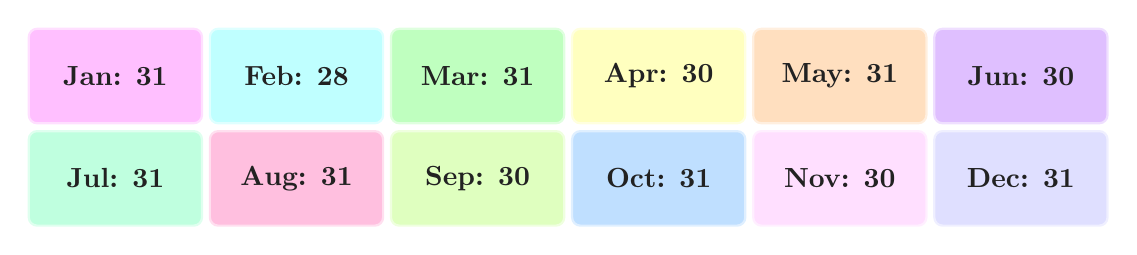
\begin{tikzpicture}
		\foreach \m[count=\i] in {Jan,Feb,Mar,Apr,May,Jun,Jul,Aug,Sep,Oct,Nov,Dec} {
				\pgfmathsetmacro{\xpos}{mod(\i-1,6)*2.3}
				\pgfmathsetmacro{\ypos}{-int((\i-1)/6)*1.3}
				\node[fill=\monthcolor{\i}, draw=\monthcolor{\i}!50, thick,
					minimum width=2.2cm, minimum height=1.2cm,
					font=\bfseries, text=darkbg, rounded corners=3pt]
				at (\xpos, \ypos) {\m: \daysofmonth{2026}{\i}};
			}
	\end{tikzpicture}

	\vspace{1.5cm}

	
\begin{tikzpicture}
		\fill[colmay] (0,0) rectangle (0.6\paperwidth, 0.8cm);
		\node[anchor=center, font=\bfseries\Large, text=darkbg, rounded corners=3pt]
		at (0.3\paperwidth, 0.4cm) {Total Days: 365};
	\end{tikzpicture}

	\vfill

	\textcolor{lighttext}{\large Generated with \LaTeX\ • Inspired by Engineering Formulasheets}

	\vspace{0.5cm}

	\textcolor{lighttext!70}{\footnotesize Colors: Each month has a unique pastel color}
\end{center}

\end{document}
